\documentclass{article}
\usepackage[russian]{babel}
\usepackage[utf8]{inputenc}
\usepackage{epsfig}
\usepackage{graphicx}
\usepackage{caption}
\usepackage{subcaption}
\usepackage{amssymb}
\usepackage{amsmath}

\DeclareMathOperator*{\argmin}{arg\,min}
\DeclareMathOperator*{\argmax}{arg\,max}

\title
    {Решение задачи MAP для марковской сети типа решётка}
\author
    {Новиков~А.\,В.\\
    МГУ, ВМиК, каф. ММП}

\begin{document}
\maketitle

\pagebreak

\section{Введение}
Марковские случайные сети (MRF) --- это популярный подход к решению задач анализа данных.
Одна из самых важных задач возникающих при использовании MRF ---
максимизации апостериорной вероятности.
Для большинства реальных задач эта задача NP--трудная.\\
В данной статье проводится обзор существующих
state-of-the-art подходов к этой задаче.

\subsection{Вклад}
Платформа для сравнения алгоритмов и выводы о перспективности тех или иных способов оптимизации.

\subsection{Обозначения}


\section{Данные}
Для сравнения подходов мы использовали данные
опубликованные Karteek Alahari~\cite{Alahari}
\pagebreak

\section{Обзор методов}
На сегодняшний день самым лучшим общим
методом решения данной задачи считается
метод Alpha--Expansion~\cite{AlphaExp}.
Мы будем сравнивать его с TRW--S~\cite{TRWS} и методами использующими
двойственное разложение. В них задача минимазации
исходной энергии\footnote{От максимизации апостериорной вероятности традиционно переходят
к минимизации минус логарифма вероятности (его называют энергией).}
сводится к задаче максимизации
двойственной энергии (это функция в отличии от исходной энергии
является вогнутой кусочно--линейной).
Алгоритмы этой группы отличает конкретный метод максимизации.


\begin{itemize}
\item Alpha--Expansion~\cite{AlphaExp}
\item TRW--S~\cite{TRWS}
\item Субградиентный подъём~\cite{Subgradient}
\item L--BFGS~\cite{BFGS}
\item Bundle methods~\cite{Bundle}
\item <<Полная декомпозиция>>
\end{itemize}
\pagebreak

\section{Постановка задачи}

\subsection{Двойственное разложение}



\section{Методы оптимизации двойственной функции}
\subsection{Субградиентный подъём}
Результаты работы данного метода зависят от выбора
последовательности шагов $\alpha_t$.
Мы сравнили константный, адаптивный шаг, неточную
одномерную оптимизация по величине шага, а так же
точную однмерную оптимизацию.\\
Адаптивный подход нашел глобальный минимум,
показав результат лучше чем $\alpha$--расширение,
но работал примерно в $60$ раз дольше.
Использование константного подхода показывает
примерно одинаковые результаты для разных констант
из хорошего диапазона. Если не угадать с константой,
то метод либо разойдётся, либо будет сходится слишком медленно.
В случае адаптивного шага использовалась следующая формула:\\
$\alpha_t = \frac{Approx_t - Dual_t}{\left \| \Delta \overrightarrow{g_t} \right \|^2}$\\
Где $Dual_t$~--- текущее значение двойственной функции, 
$Approx_t$~--- оценка оптимума двойственной функции.\\
$Approx_t = BestDual_t + \delta_t$,\\
где $BestDual_t$~--- лучшее на данный момент значение двойственной функции,\\
\begin{equation}
    \delta_{t+1} = \begin{cases}
    \gamma_0 \delta_t, & Dual_t > Dual_{t-1},\\
    max(\gamma_1 \delta_t, \epsilon) & Dual_t \leqslant  Dual_{t-1}.
    \end{cases}
\end{equation}
$\gamma_0$, $\gamma_1$, $\epsilon$~--- параметры метода, выбранные нами эмпирически.\\
$\gamma_0 = 1.5$\\
$\gamma_1 = 0.5$\\
$\epsilon_t = \frac{1}{t}$\\


\begin{figure}
    \centering
    \begin{subfigure}[t]{\textwidth}
            \centering
            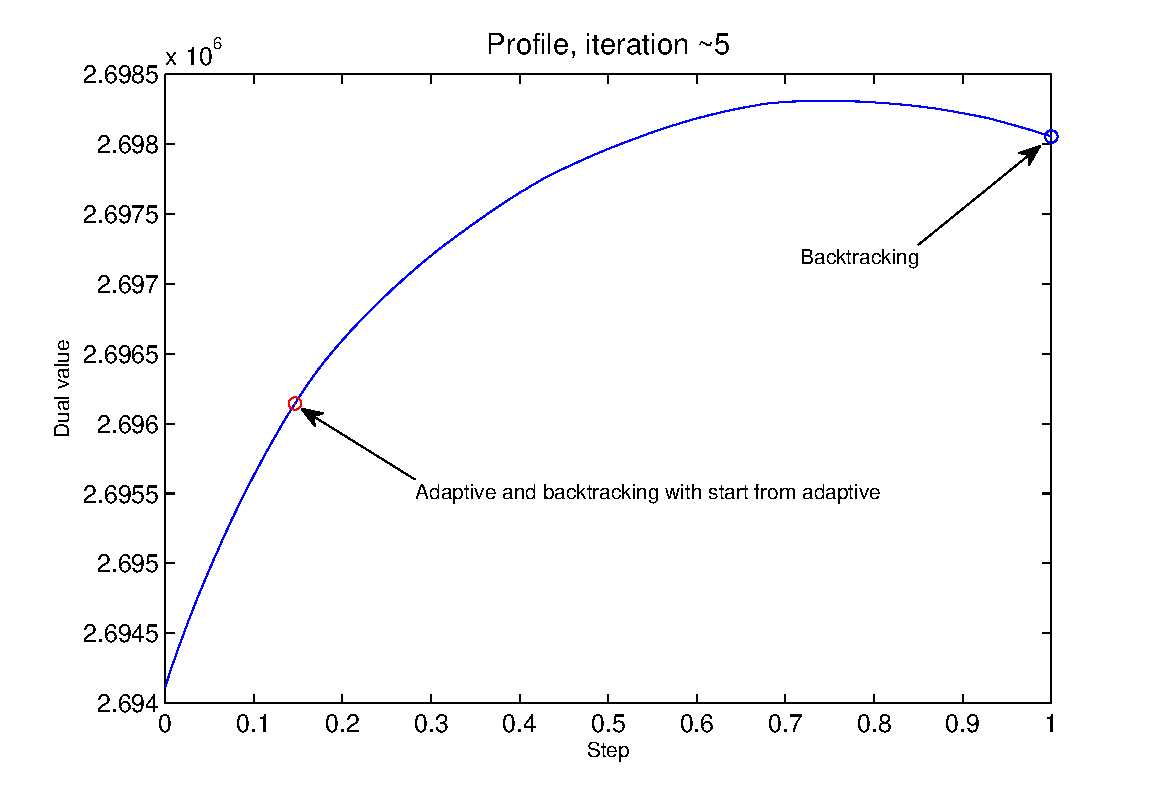
\includegraphics[width=0.9\textwidth]{profile_tsukuba.eps}
    \end{subfigure}
    \begin{subfigure}[t]{\textwidth}
            \centering
            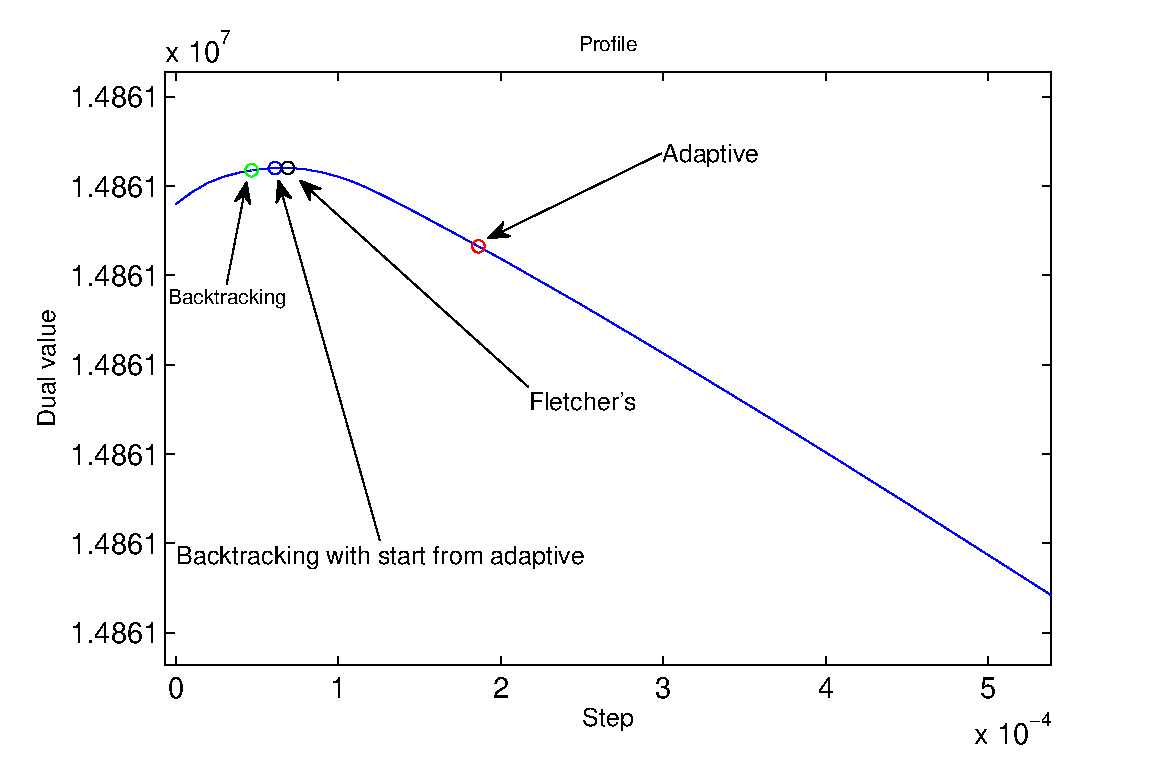
\includegraphics[width=0.9\textwidth]{profile_cones.eps}
    \end{subfigure}
    \caption{Профиль двойственной функции вдоль направления оптимизации и неточные максимумы найденные различными алгоритмами}
    \label{fig:profile}
\end{figure}
Не смотря на то, что двойственная функция является кусочно линейной, она очень близка к гладкой, так что методы неточной одномерной оптимизации кажутся довольно перспективным направлением работы~(рис.~\ref{fig:profile}). Нами был опробован метод Флетчера и <<backtracking>>.\\


На графиках приведены примеры работы алгоритмов (в том числе
длинны шагов, выбранных адаптивным методом) на стереопаре Tsukuba.
\begin{figure}
    \centering
    \begin{subfigure}[t]{\textwidth}
            \centering
            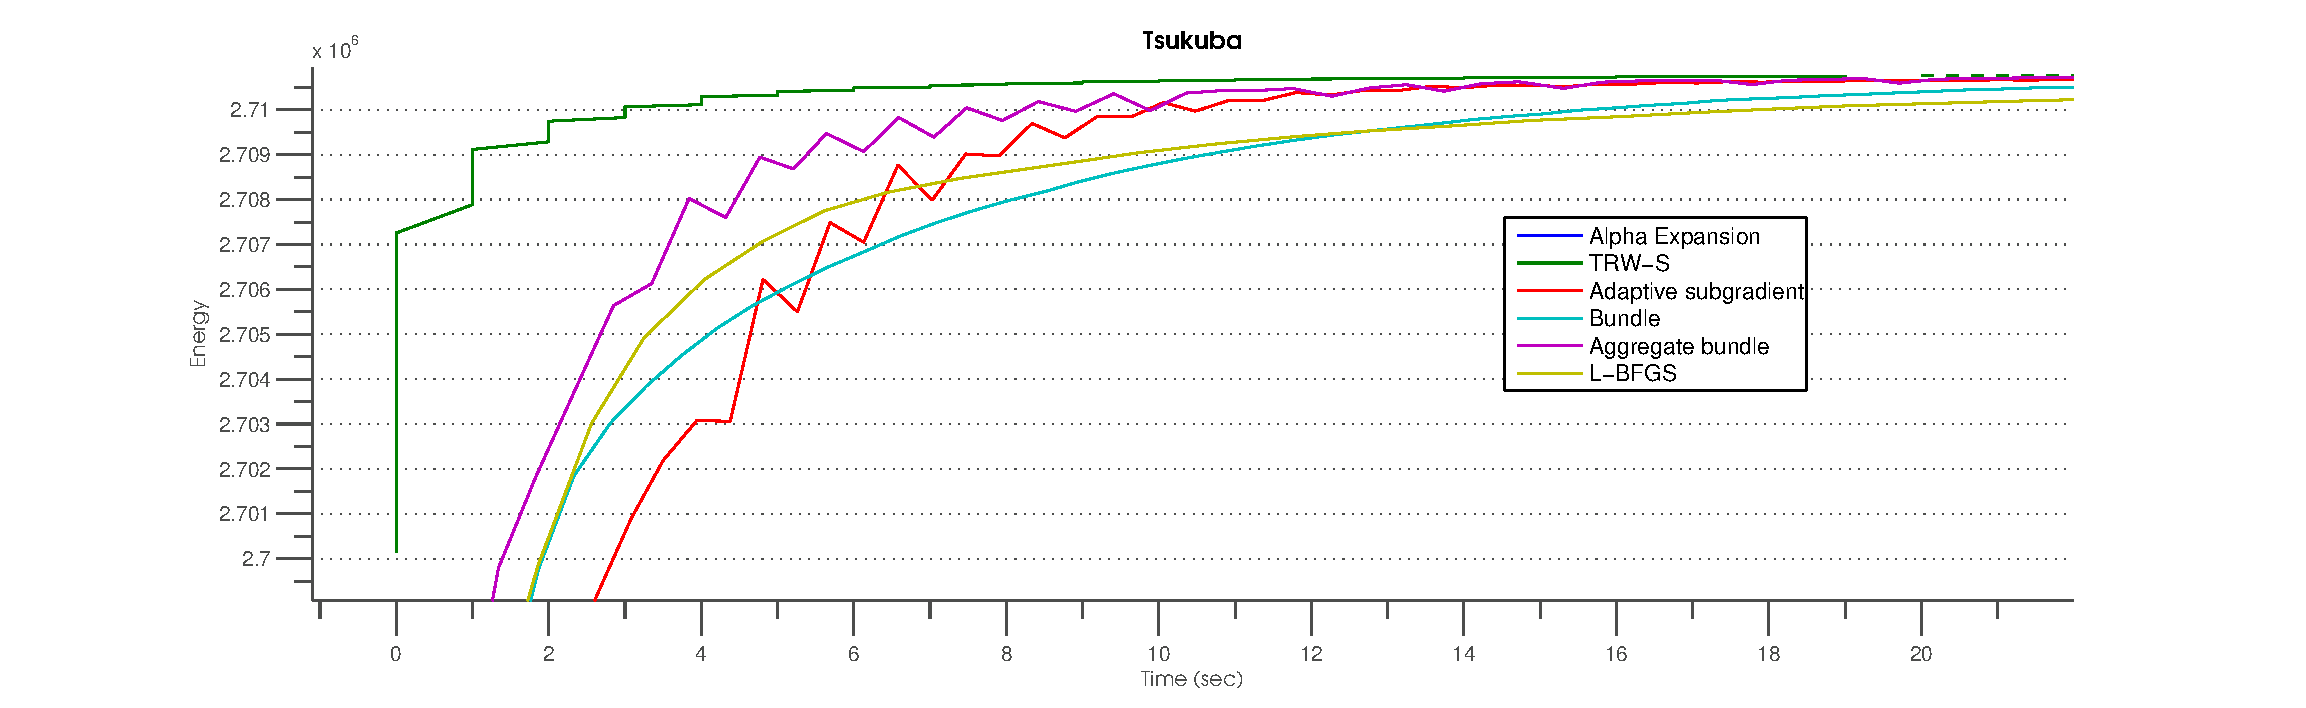
\includegraphics[width=1.5\textwidth]{comparative_tsukuba.eps}
            \caption{Сравнение скорости и качества работы различных методов.
                    Для $\alpha$--расширения указанна только прямая энергия,
                    для остальных алгоритмов указанна прямая и двойственная энергия.}
    \end{subfigure}
    \begin{subfigure}[t]{\textwidth}
            \centering
            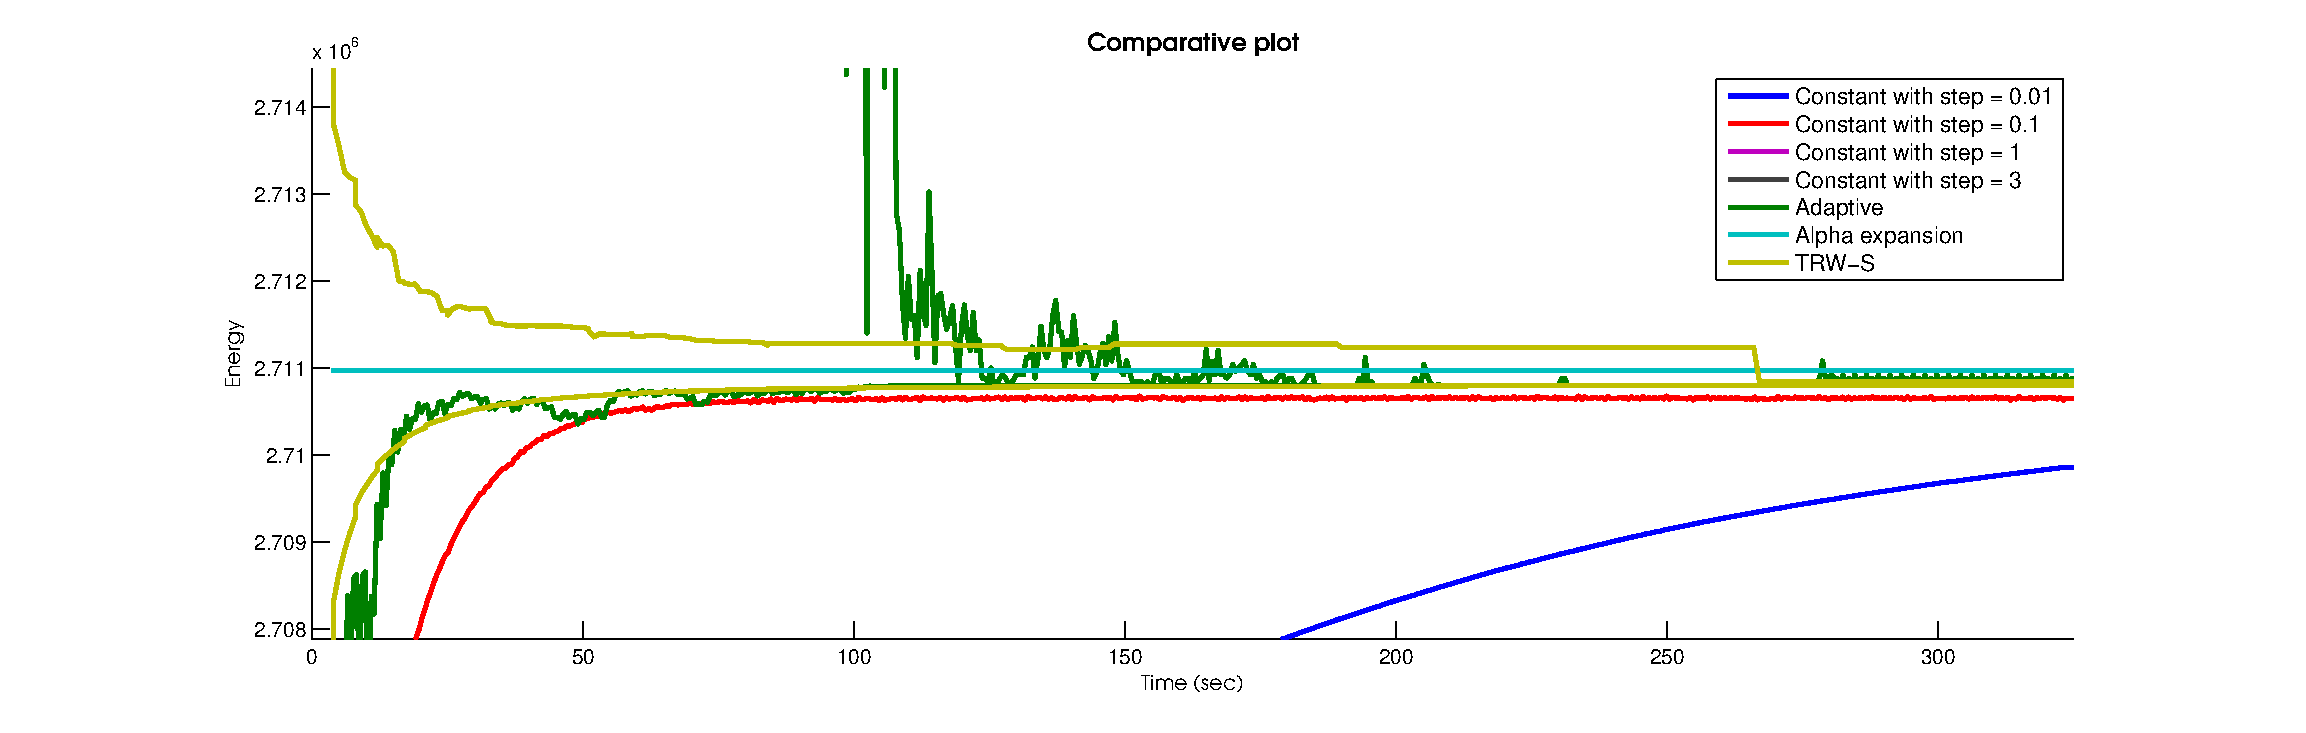
\includegraphics[width=1.5\textwidth]{comparative_tsukuba_small.eps}
    \end{subfigure}
    \begin{subfigure}[t]{\textwidth}
            \centering
            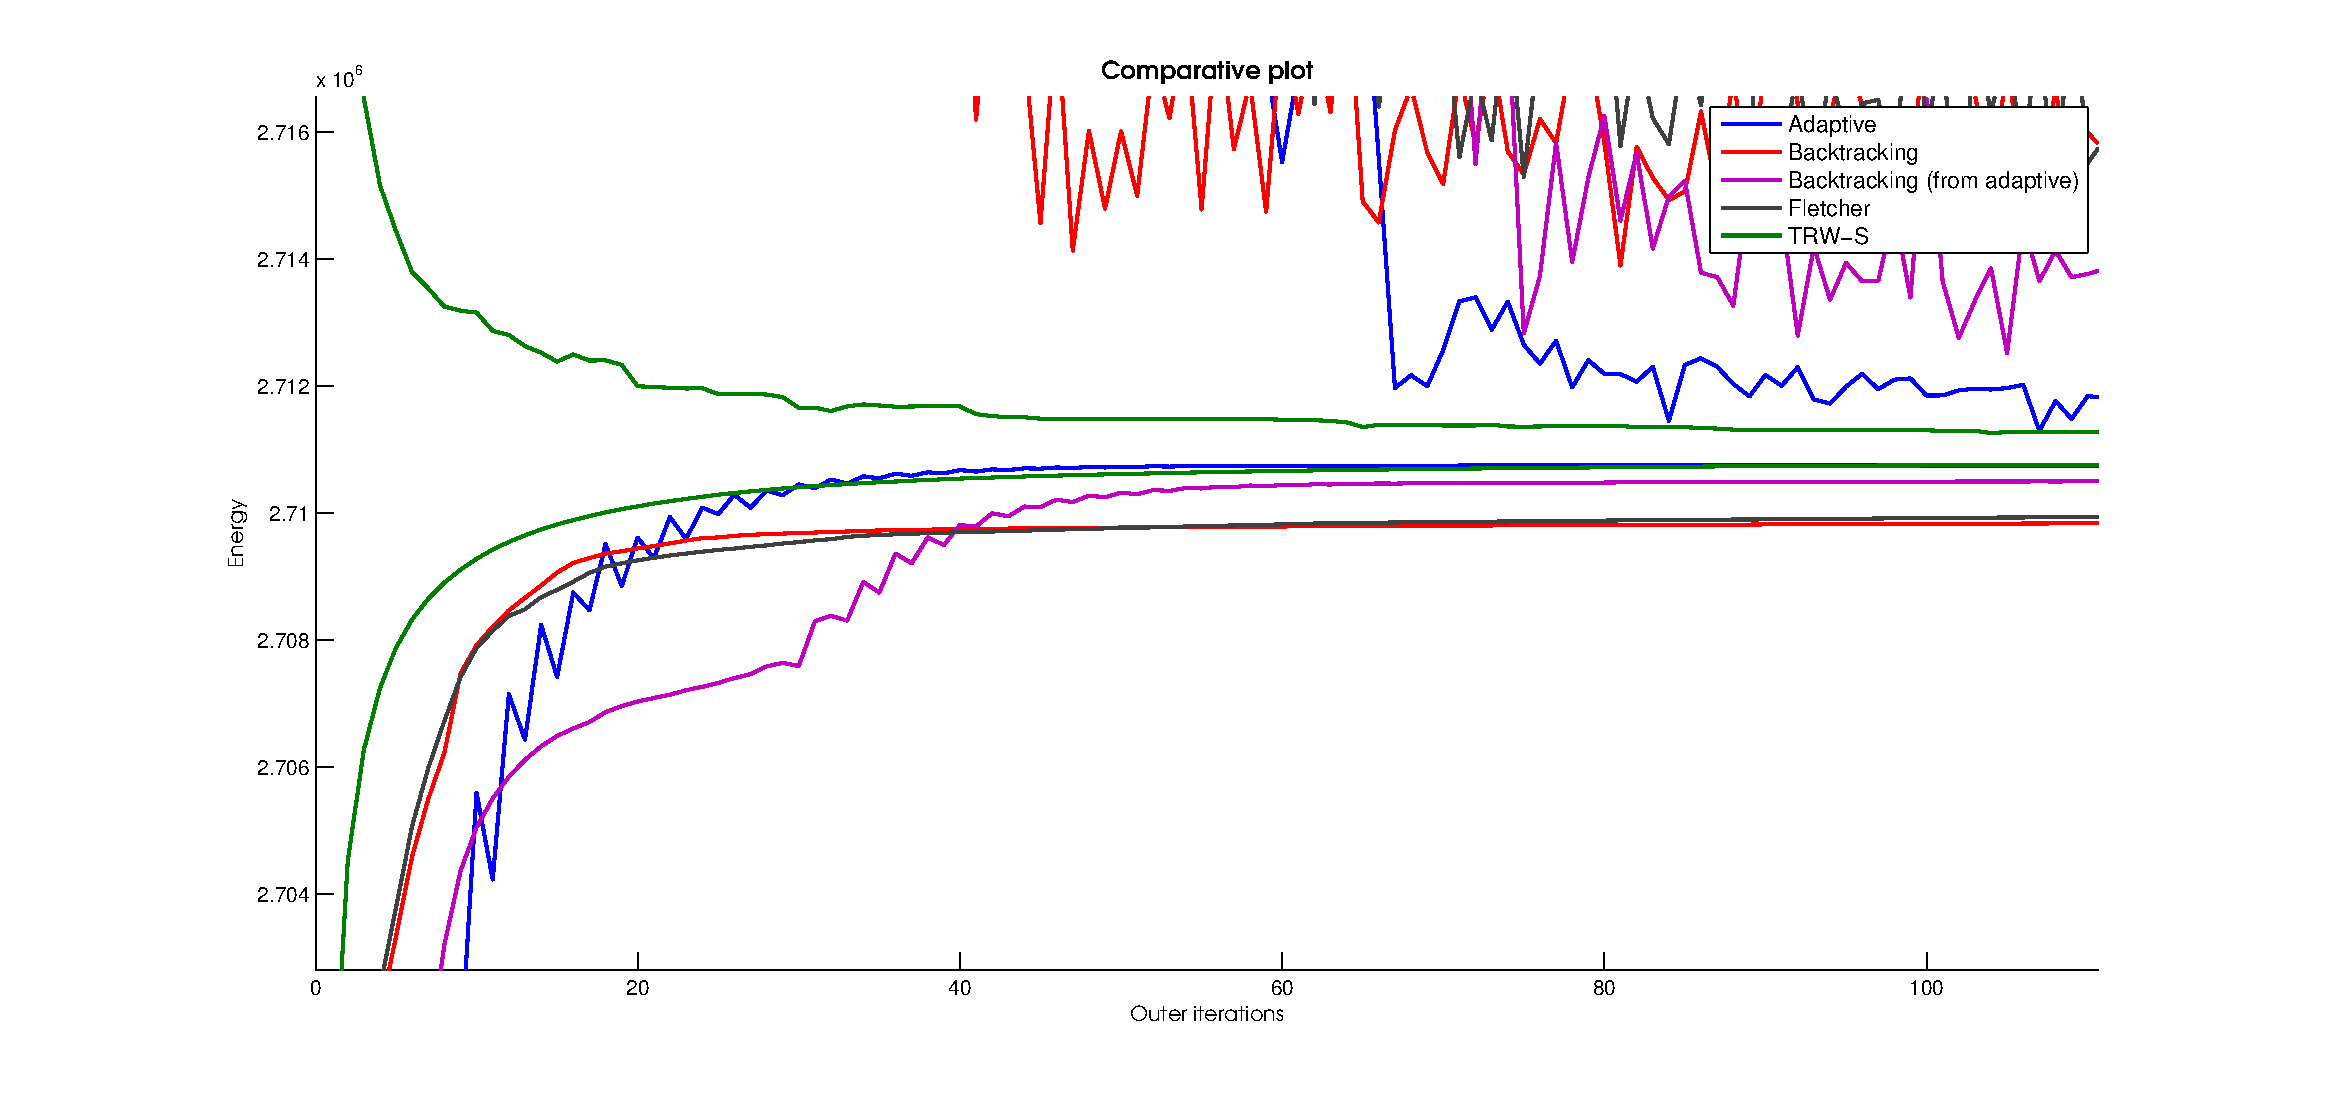
\includegraphics[width=1.5\textwidth]{1d_optimization.eps}
    \end{subfigure}
\end{figure}

\begin{figure}
    \centering
    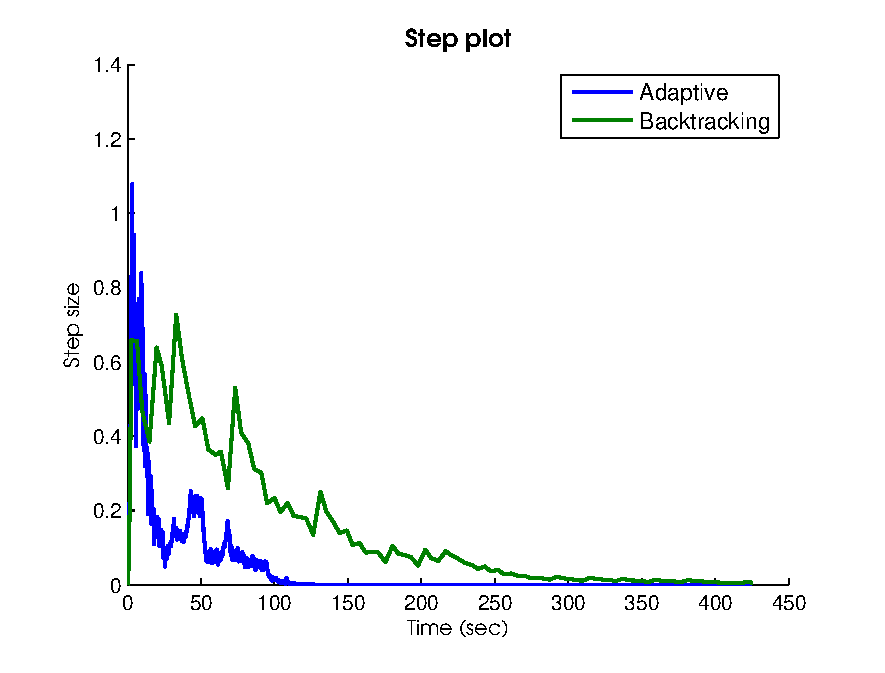
\includegraphics[width=\textwidth]{step_adap_vs_adapBack.eps}
    \caption{Длинна шага выбранная на каждой итерации адаптивным методом и методом <<backtracking>>}
\end{figure}

\begin{figure}
    \centering
    \begin{subfigure}[t]{\textwidth}
            \centering
            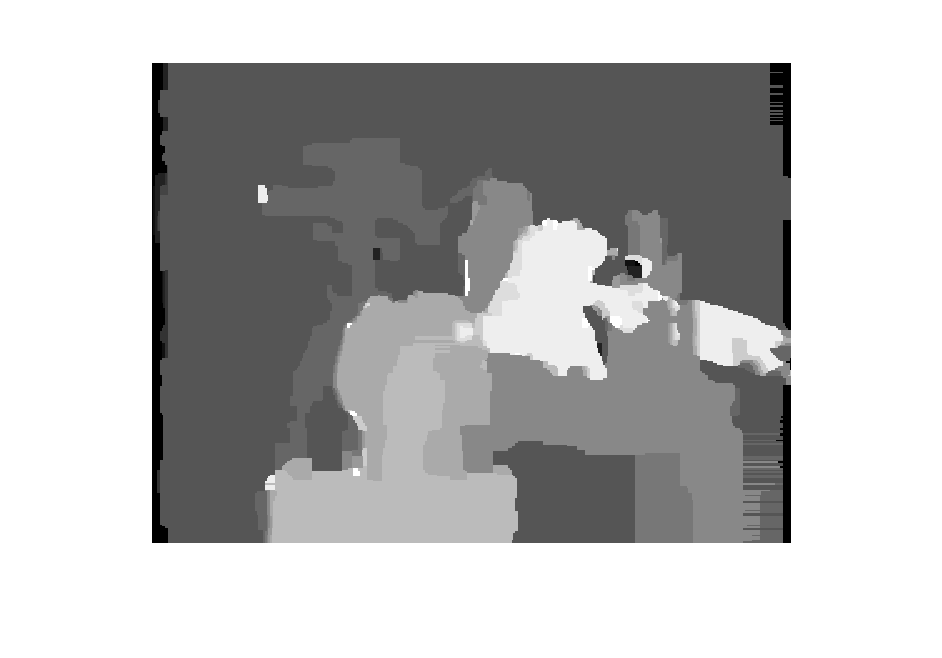
\includegraphics[width=\textwidth]{adaptive_result.eps}
            \caption{Итоговая разметка выбранная наилучшим методом (адаптивным)}
    \end{subfigure}
    \begin{subfigure}[t]{\textwidth}
            \centering
            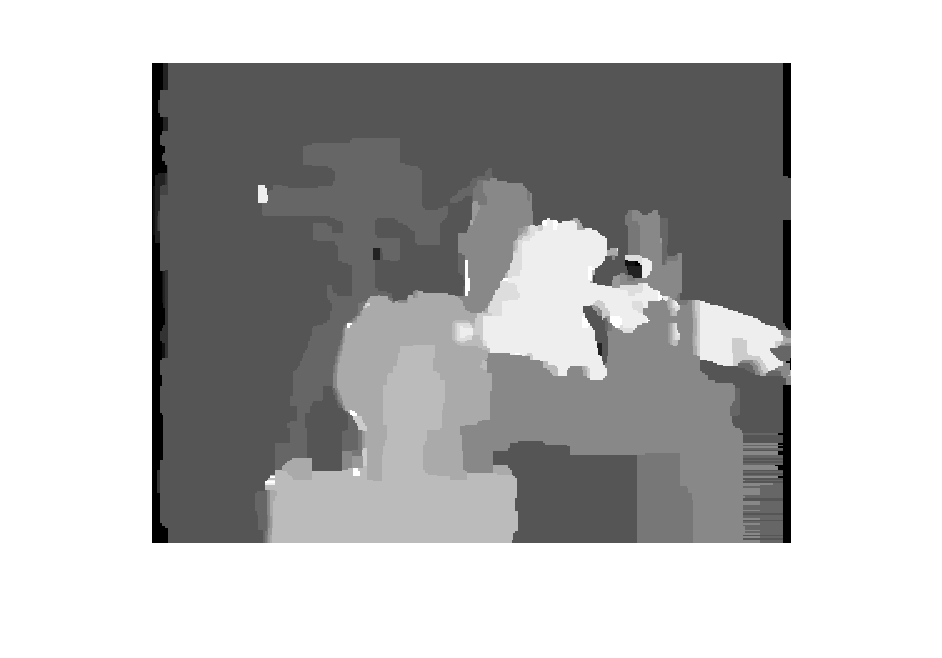
\includegraphics[width=\textwidth]{constant_0_1_result.eps}
            \caption{Разметка выбранная константным методом с длинной шага $0.1$}
    \end{subfigure}
\end{figure}


\subsection{Bundle методы}
Основная идея bundle методов --- ограничить двойственную функцию $f(\lambda)$ сверху с помощью вогнутой кусочно--линейной функции $\hat{f}(\lambda)$ и дальше оптимизировать (уточняя на каждом шаге) именно $\hat{f}(\lambda)$. Эта функция строится по последовательности точек $\{\lambda_i\}$, значений в этих точках $\{f(\lambda_i)\}$ и субградиентов $g^i \in \partial f(\lambda_i)$ так, что $f(\lambda) \leq \hat{f}(\lambda)$ и $f(\lambda_i) = \hat{f}(\lambda_i)$. Вместе $\{\lambda_i\}$, $\{f(\lambda_i)\}$ и  $g^i \in \partial f(\lambda_i)$ составляют \textit{bundle} $\mathcal{B}$.
\begin{equation}
\hat{f}(\lambda) = \min_{(\lambda{}', f(\lambda{}'), g{}') \in \mathcal{B}} \{f(\lambda{}') + <g{}', \lambda - \lambda{}'>\}
\end{equation}

Для генерации последовательности точек мы используем проксимальный алгоритм:\\
\begin{equation}
\lambda^{k + 1} = \argmax_{\lambda} \{\hat{f}(\lambda)  - \frac{w^k}{2} \left \| \lambda - \overline{\lambda} \right \|_2^2\}
\end{equation}
где $w^k > 0$ нужен чтобы удержать $\lambda^{k + 1}$ около текущего кандидата на решение ($\overline{\lambda}$), где $\hat{f}(\lambda)$ близок к $f(\lambda)$. По смыслу данный параметр соотствует величене обратной длине шага.\\
Если новая точка $\lambda^{k + 1}$ не ведет к значительному прогрессу, мы не меняем текущую оценку решения $\overline{\lambda}$, а только уточняем $\hat{f}(\lambda)$ добавляя в bunble $(\lambda^{k+1}, f(\lambda^{k+1}), g^{k+1})$. $k$--ый шаг в таком случае называют \textit{нулевым шагом}. В противном случае мы обновляем $\overline{\lambda} = \lambda^{k + 1}$, это называется \textit{значительным шагом}. Чтобы понять какой вид шага нужно выполнять сейчас мы сравниваем увеличение $f(\lambda^{k+1})$ и $\hat{f}(\lambda^{k+1})$ относительно $f(\overline{\lambda})$. Если отношение этих величин больше чем заранее зафиксированный параметр $m_L$, тогда аппроксимация $\hat{f}(\lambda)$ достаточно точна чтобы предпринять значительный шаг.\\


В описанном алгоритме осталось два аспекта сильно влияющих на итоговую скорость оптимизации --- это управление размером бандла $\mathcal{B}$ (бандл должен быть достаточно маленьким чтобы можно было быстро решать задачу квадратичного программирования возникающую на каждой итерации) и выбор последовательности весов $\{w^k\}$.

\subsubsection{Управление размером бандла}

\subsection{L-BFGS}


\section{Сравнение подходов}

\section{Выводы}

\begin{thebibliography}{1}
\bibitem{TRWS}
    {Kolmogorov~V.}
    {Convergent Tree-Reweighted Message Passing for Energy Minimization}~//
    {IEEE} Trans. Pattern Anal. Mach. Intell., 2006.~--- С.\,1568--1583.
\bibitem{ABundle}
    {Kiwiel~K.}
    {An aggregate subgradient method for nonsmooth convex minimization}~//
    Mathematical Programming, 1983, 27:320--341.
\bibitem{Alahari}
    {Alahari~K., Kohli~P., Torr~P.~H.~S.}
    {Dynamic Hybrid Algorithms for MAP Inference in Discrete MRFs}~//
    {IEEE} Trans. Pattern Anal. Mach. Intell., 2010.~--- С.\,1846--1857.
\bibitem{Subgradient}
    {Komodakis~N., Paragios~N., Tziritas~G.}
    {MRF energy minimization and beyond via dual decomposition}~//
    Pattern Analysis and Machine Intelligence, IEEE Transactions on, 2011.~--- С.\,531--552.
\bibitem{Bundle}
    {Kappes~J.\,H., Bogdan~Savchynskyy, Christoph~Schnorr}
    {A Bundle Approach To Efficient MAP-Inference by Lagrangian Relaxation}~//
    Computer Vision and Pattern Recognition (CVPR), IEEE Conference 2012.~--- С.\,1688--1695.
\end{thebibliography}
\end{document}

